[TODO: Detallar todo el proceso de implementación]

\subsection{Conjunto de entrenamiento}
[TODO: Creación del dataset básico]

\subsubsection{FAQS}
30 variaciones por pregunta, faltas de otrografia, etc

\subsubsection{Chachara}
Preguntas basicas

\subsubsection{Out of scope}
\cite{bestPracticesNLU}


\subsubsection{Patrones de conversación}
Respuestas basicas, gracias, saludos, necesitas ayuda etc

\subsection{Aplicación web}
Desarrollo del frontend

\subsection{Despliegue}
Una vez implementados el servidor y el \textit{frontend} web es necesario publicar una versión de prueba del servicio para poder empezar con la fase de obtención de datos de conversaciones reales. Para ello, la Universitat Politècnica de València pone a disposición del proyecto una maquina virtual con \textit{Ubuntu 18.04} donde poder realizar el despliegue. Mediante acceso \textit{SSH} se instalan todas las librerías necesarias (\textit{apache}, \textit{python}, \textit{rasa}, \textit{spacy} etc) y se ponen en marcha tanto la web como el servidor conversacional.\\

Una vez el sistema está funcionando se realiza una pequeña prueba para asegurarse que la recogida de datos funciona correctamente. Tras un resultado satisfactorio se solicita a la universidad la apertura de los puertos 80, 5055 y 5005 para que los usuarios externos puedan acceder y probar el chatbot.\\


\subsection{Desarrollo basado en conversaciones}
El desarrollo basado en conversaciones (\textit{Conversation-Driven Development}) es el proceso de escuchar a los usuarios y utilizar esa información para mejorar el asistente \cite{conversationDriven}. Programar chatbots robustos puede ser un auténtico reto pues los usuarios siempre dirán algo que inicialmente no estaba previsto. En consecuencia, este enfoque es la mejor manera de desarrollar un chatbot y está especialmente recomendado por los desarrolladores de \textit{Rasa} \cite{bestPracticesNLU}.\\

Tras publicar la primera versión de prueba del chatbot el proyecto se encuentra listo para entrar en esta fase de desarrollo centrada en la recogida de datos. Para ello, durante varias semanas se compartirá el chatbot, se revisarán las conversaciones obtenidas, y se anotarán, clasificarán e incorporarán al \textit{dataset} todos los datos recopilados. Tras realizar todos estos cambios sobre el conjunto de entrenamiento se ejecutarán los \textit{tests} correspondientes, se corregirán posibles errores y se volverá a compartir el chatbot para una nueva iteración.\\

\begin{figure}[htbp]
\centering
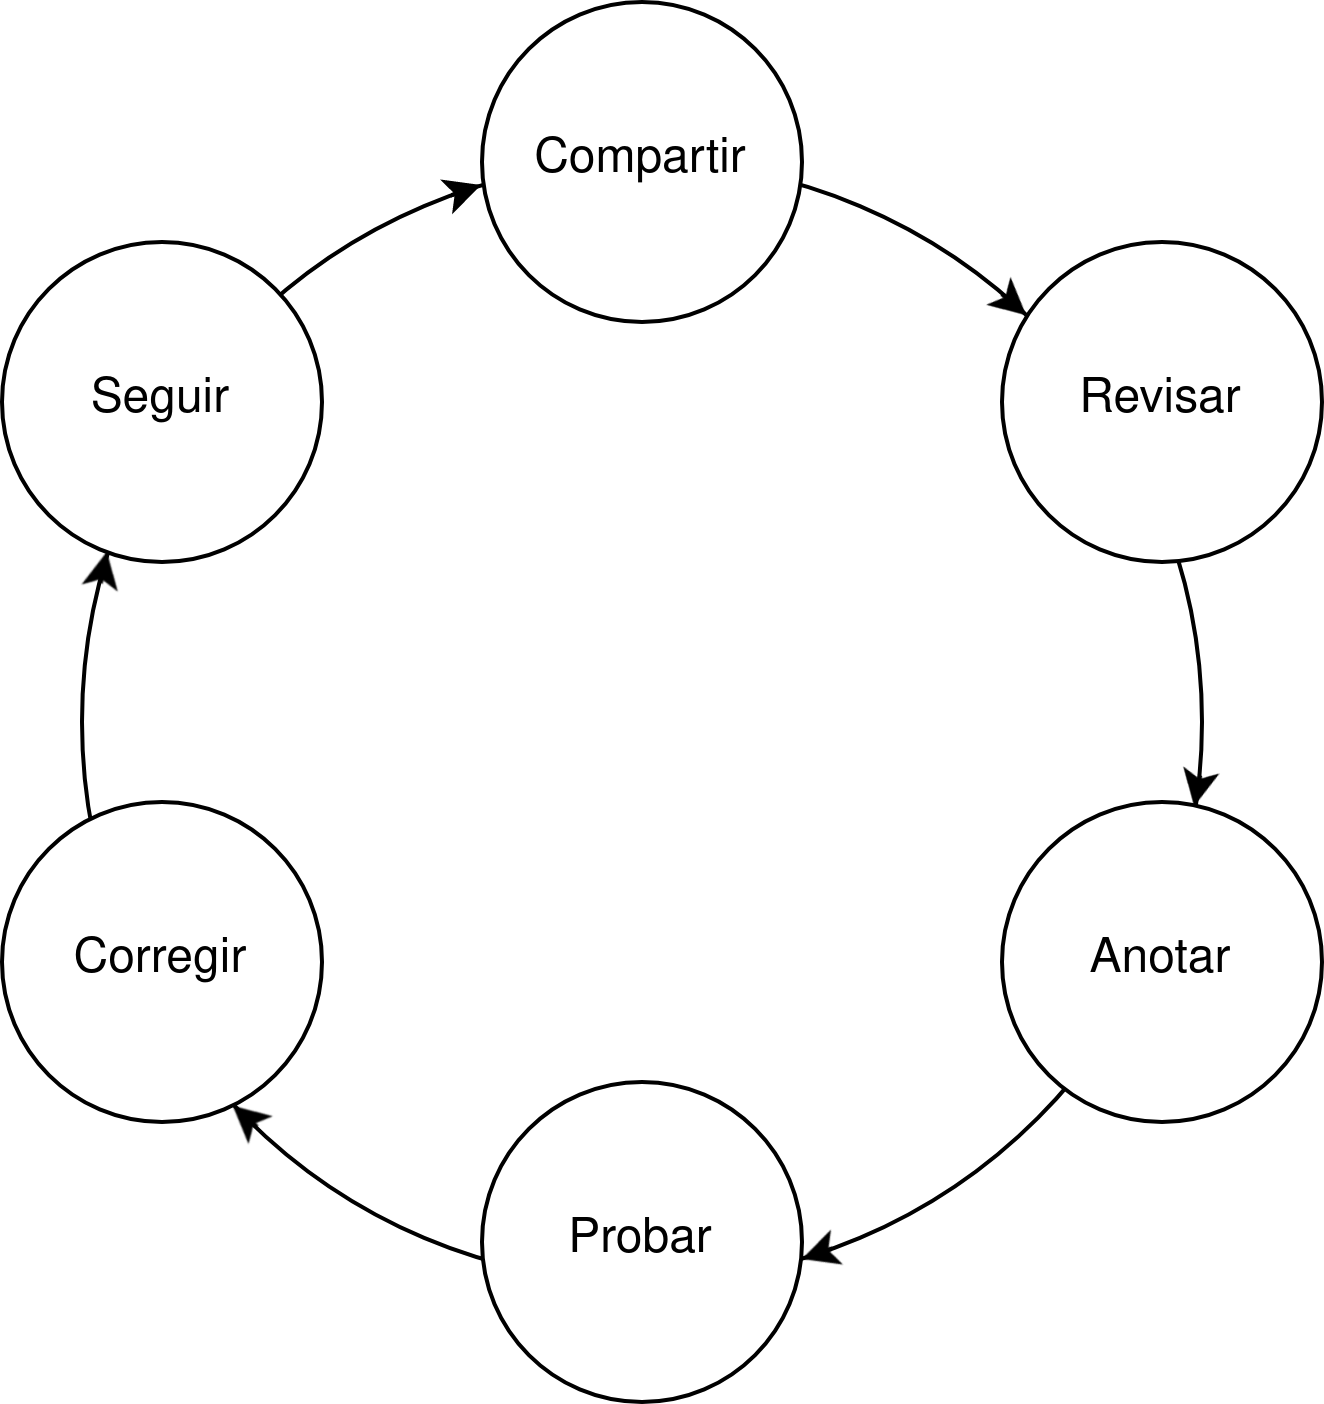
\includegraphics[scale=0.15]{../images/cdd.png} 
\caption{Ciclo del desarrollo basado en conversaciones}
\label{fig:cdd}
\end{figure}

Se trata de etiquetar, clasidficar, encontrar fallos, flowas ...\\	

\begin{figure}[htbp]
\centering
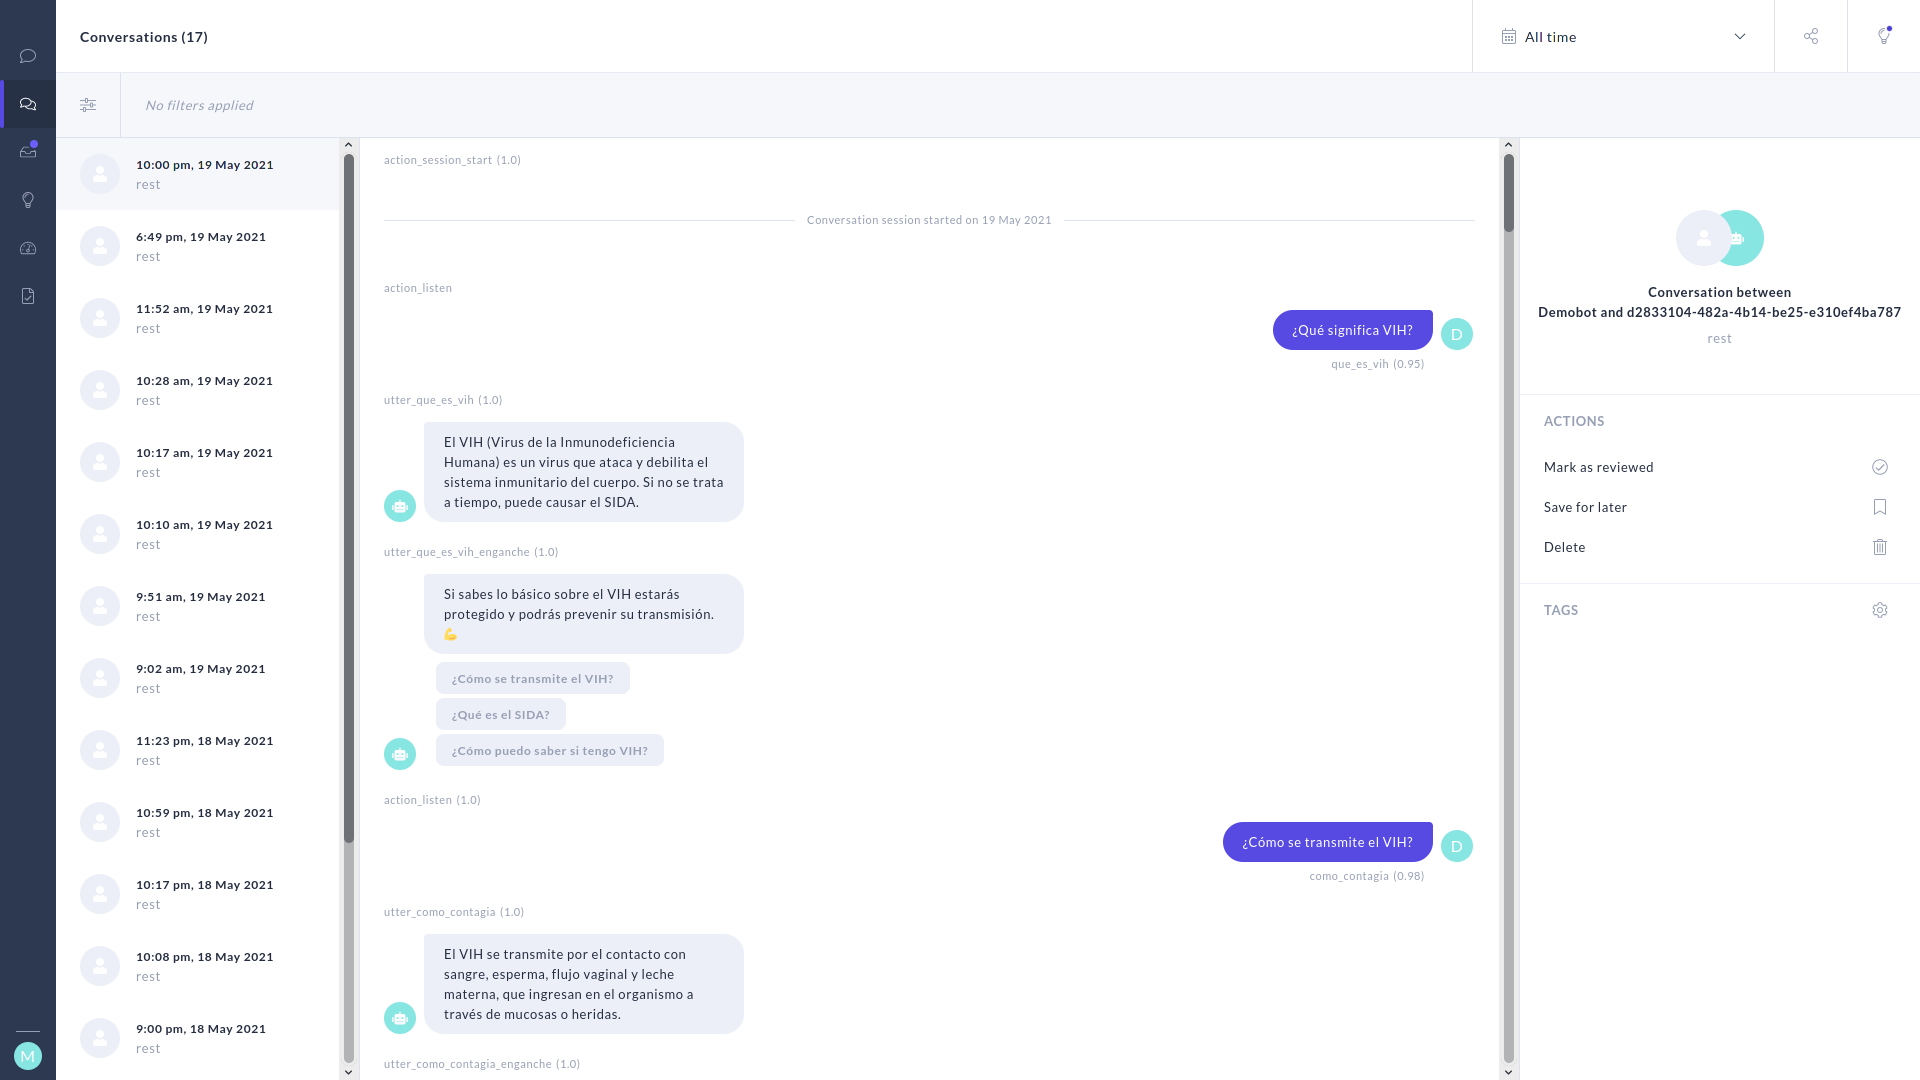
\includegraphics[scale=0.3]{../images/collected_dialogs.png} 
\caption{Ejemplo de una de las conversaciones recogidas}
\label{fig:collected dialogs}
\end{figure}

Durante todo este proceso se recogieron y analizaron aproximadamente 23 conversaciones de las cuáles se pudo extraer e incorporar a la base de conocimiento la siguiente información:\\

\begin{itemize}
	\item 30 preguntas nuevas que inicialmente no estaban previstas.
	\item 204 datos NLU
\end{itemize}


\begin{figure}[htbp]
\centering
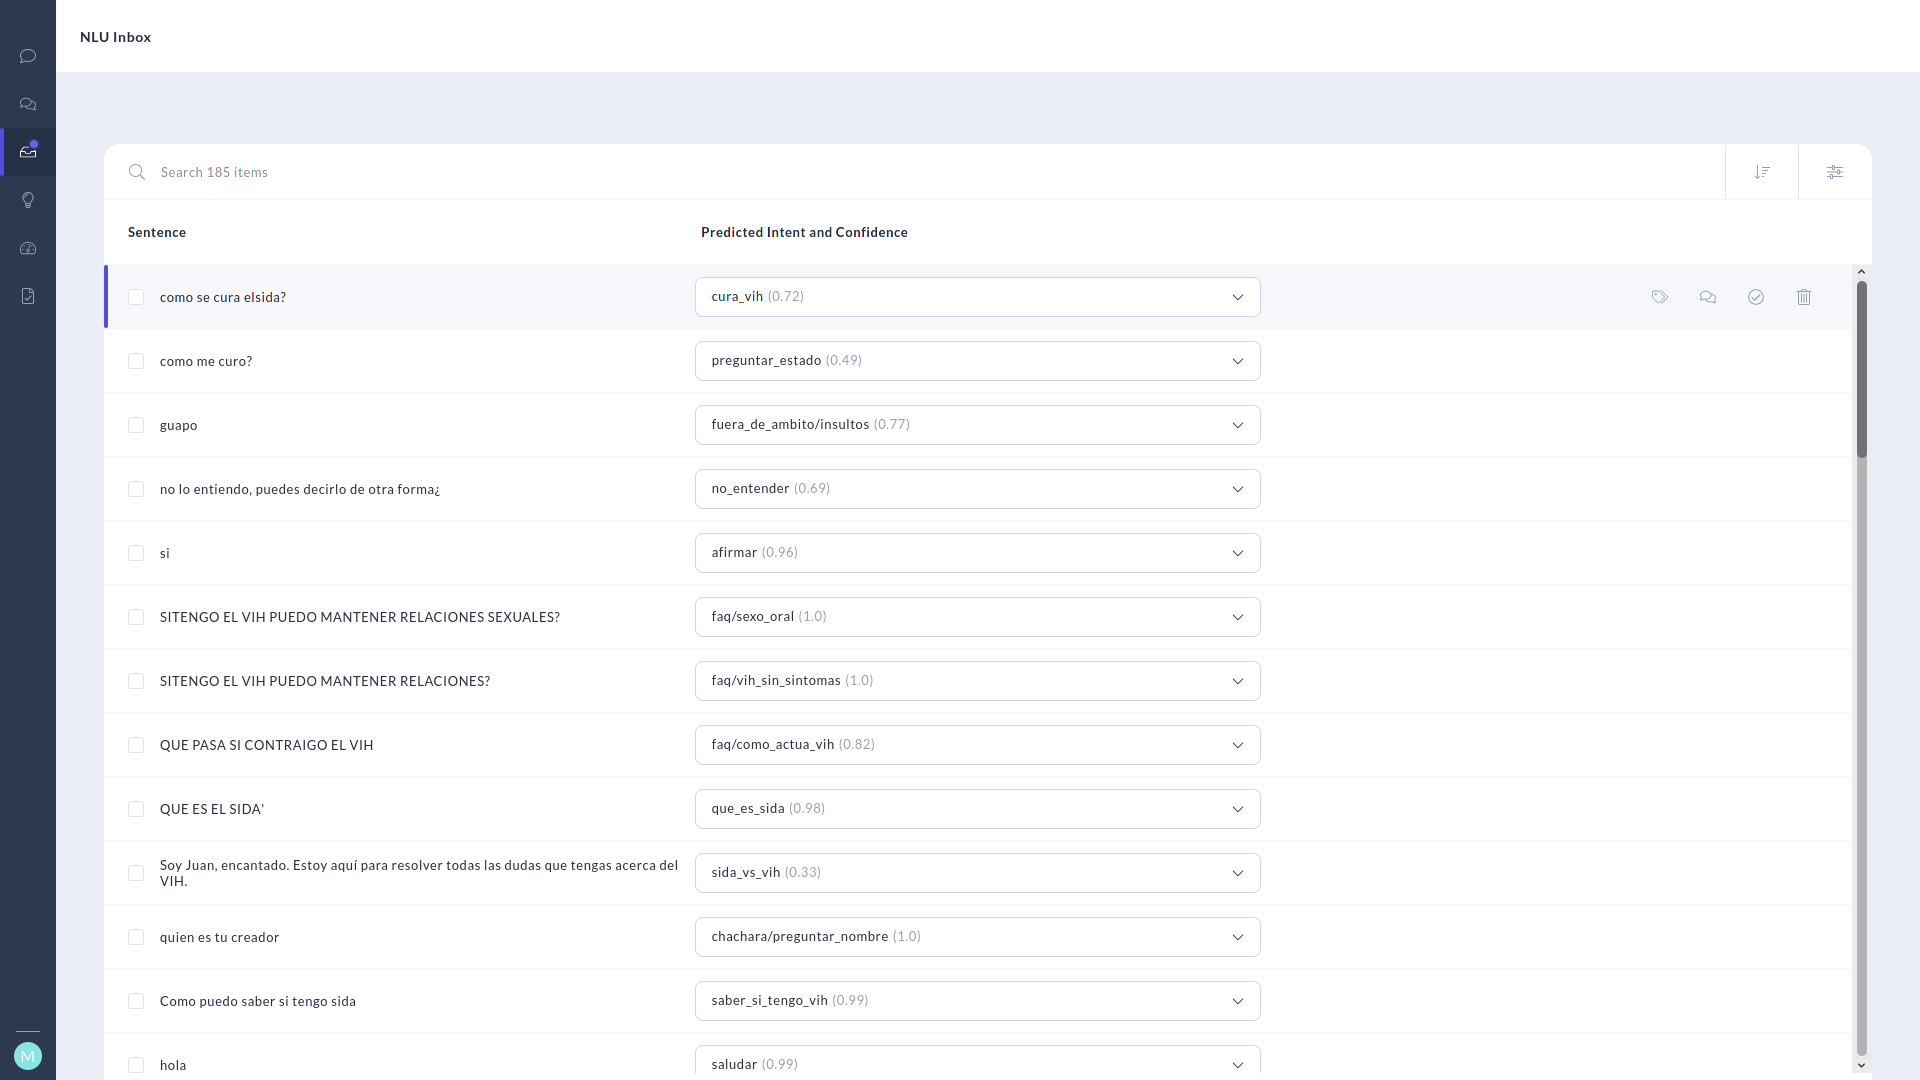
\includegraphics[scale=0.3]{../images/collected_nlu.png} 
\caption{Datos NLU recopilados y su etiquetado}
\label{fig:collected nlu}
\end{figure}




[TODO: Recogida de conversaciones reales y etiquetado]
